
\section{Zielsetzung}
Ziel des Versuches ist es, sich mit der Erzeugung und Leitung von Mikrowellen vertraut zu machen.
Dazu werden insbesondere die Eigenschaften bei der Leitung über Hohlleiter untersucht.

\section{Theorie}
Als Mikrowellen werden elektromagnetische Wellen im Wellenlängenbereich zwischen einigen $\si{\milli\meter}$
und ca. $\SI{10}{\centi\meter}$ bezeichnet. Dies entspricht einem Frequenzbereich von etwa
$\SI{1}{\giga\hertz}$ bis $\SI{300}{\giga\hertz}$.  Da diese Frequenz zu hoch für einen gewöhnlichen
Schwingkreis ist, erfolgt die Erzeugung von Mikrowellen über Klystrons, Wanderfeldröhren oder Magnetrons.

\subsection{Das Reflexklystron}
Eine spezielle Art des Klystrons ist das Reflexklystron, dessen Aufbau schematisch in Abbildung \ref{fig:kly}
dargestellt.
\begin{figure}[H]
  \centering
  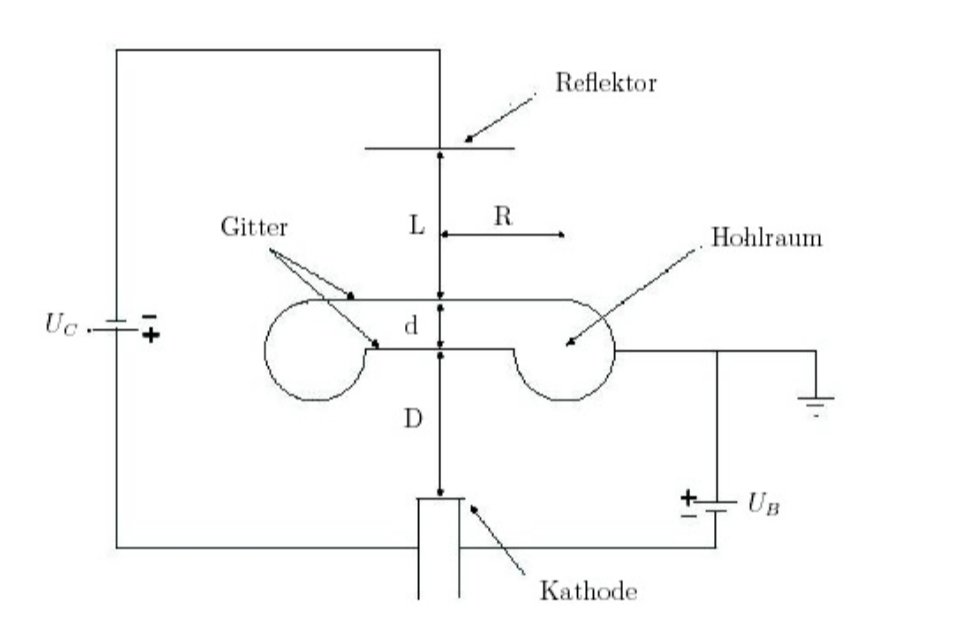
\includegraphics[height=12cm]{kly.png}
  \caption{Schematischer Aufbau eines Reflexklystrons \cite{Kly}.}
  \label{fig:kly}
\end{figure}
Es besteht grundlegend aus einem Hohlraumresonator, einem Resonator und einer Kathode.
Durch Erhitzen der Kathode emmitiert diese freie Elektronen, da die Austrittsarbeit durch die thermische
Energie geleistet wird. Diese freien Elektronen werden durch die Beschleunigungsspannung $U_1$ in Richtung
des positiv geladenen Hohlraumresonators beschleunigt. Durch Gitter im Boden und im Deckel kann der Elektronenstrahl
in den Resonator ein und anschließend auch wieder austreten. Zwischen diesen Gittern liegt ein elektrisches
Wechselfeld an, welches die Elektronen je nach Zeitpunkt des Eintritts die Elektronen entweder beschleunigt oder
abremst. Dieser Vorgang wird als Geschwindigkeitsmodulation bezeichnet. Zwischen dem oberen Gitter und dem
Reflektor liegt ebenfalls eine Spannung an, welche auch als Reflektorspannung bezeichnet wird. Da der Reflektor negativ
geladen ist, ist diese umgekehrt zur Strahlspannung gepolt und führt folglich zu einer Richtungsumkehr der
Elektronen, welche nach Durchlaufen des Hohlraumresonators aus dem Gitter austreten. Die Weglänge, die die
Elektronen im Reflektorraum beim Anlaufen gegen die Reflektorspannung zurücklegen können ist abhängig von der kinetischen
Energie der Elektronen. Elektronen, die zuvor im Hohlraumresonator beschleunigt wurden besitzen mehrn kinetische
Energie und haben demnach eine längere Weglänge und somit auch eine längere Aufenthaltszeit in dem Reflektorraum
als jene, die zuvor abgebremst wurden. Dies führt insgesamt dazu, dass alle Elektronen zusammen als
Bündel wieder zum Hohlraumresonator zurückkehren und gemeinsam in diesen eintreten. Geschieht dies zu einem
Zeitpunkt, in dem das elektrische Feld der Bewegung der Elektronen entgegengesetzt ist, werden diese abgebremst
und geben somit ihre kinetische Energie an das elektromagnetische Feld ab, welches dadurch verstärkt und
Aufrechterhalten wird. \\
Diese Verstärkung findet jedoch nur statt, wenn die Laufzeit im richtigen Verhältniss zur Schwingungsfrequenz des
Hohlraumresonators steht, was durch Abstimmung der Strahlspannung und der Reflektorspannung gewährleistet wird.
Die Verstärkung ist maximal, wenn die Laufzeit $n+\frac{3}{4}$ Perioden entspricht, mit $ n \in \symbb{N}$.
Neben der Anpassung von Reflektorspannung und Strahlspannung kann die Frequenz auch durch Änderung des
Volumens verändert werden, da somit die Kapazität und Induktivität des Hohlraumresonator und damit die
Eigenfrequenz angepasst werden. \\
Die Abkopplung der somit erzeugten elektromagnetischen Wellen erfolgt schlussendlich induktiv über einen Draht an der
Seitenwand des Hohlraumresonators. Anschließend können sie beispielsweise über einen Hohlleiter weitergeleitet werden.


\subsection{Eigenschaften des Hohlleiters}

Hohlleiter bestehen prinzipiell aus einem Metallrohr mit meist rechteckigem Querschnitt, wobei die
Metallwände in guter Näherung als ideale Leiter angesehen werden können. Mit ihnen können
Mikrowellen mit sehr geringen Verlusten transportiert werden. \\
Die Leitung basiert darauf, dass die Wellen schräg auf die Seitenflächen fallen und dabei reflektiert werden.
Für die Tangentialkomponente des elektrischen Feldes an der Metallwand ergibt sich $E_{tan}=0 $ und für die
Normalkomponente des magnetischen Feldes $H_{norm}=0$. Sind die Seitenlängen des Querschnitts $a$ und $b$,
erbibt sich durch diese Randbedingung bei ebenen Wellen die Bedingung
\begin{equation}
  k_x = \frac{m\pi}{a} \:, \: m \in \symbb{N} \\
  k_y = \frac{n\pi}{b} \:, \: n \in \symbb{N}
  \label{eqn:Bwv}
\end{equation}
an die Komponenten $k_x$ und $k_y$ des Wellenvektors.
Hieran sieht man, dass nur ein diskretes Spektrum an Wellen erlaubt ist, welche auch als Moden bezeichnez werden.
Somit folgt
\begin{equation}
  k^2 = k_x^2 + k_y^2 + k_z^2 \\
  \iff k_z = \pm \sqrt{k^2-(k_x^2 + k_y^2)} = \sqrt{k^2-k_c^2}
  \label{eqn:wellenv}
\end{equation}
mit
\begin{equation}
  k_c^2=k_x^2 + k_y^2= \Bigl(\frac{m\pi}{a}\Bigr)^2 + \Bigl(\frac{n\pi}{b}\Bigr)^2 \:.
  \ref{eqn:Wellenvektor}
\end{equation}
Für $k>k_c$ ergibt sich ein reelles $k_z$, welches eingesetzt in die Wellengleichung
\begin{equation}
  E=E_0 \text{sin}(k_xx)\text{sin}(k_yy)\text{exp}(i(k_zz-\omega t))
  \label{eqn:Wellengleichung}
\end{equation}
eine Schwingung ergibt, also wird die Welle in diesem fall geleitet. Für $k<k_c$ wird
$k_z$ jedoch imaginär und die Wellengleichung beschreibt eine exponentielle Dämpfung,
sodass sich die Welle in z-Richtung nicht mehr ausbreiten kann und die Leitung somit unterdrückt wird.
Die Frequenz $\nu_c = \frac{c}{2\pi}k_c$ wird daher kritische Wellenlänge genannt, denn
für Frequenzen unterhalb dieser kritischen Frequnz findet demnach keine
Weiterleitung mehr statt. Die entsprechende kritische Wellenlänge
\begin{equation}
  \lambda_c = \frac{c}{\nu_c}=\frac{2\pi}{k_c} =\frac{2\pi}{\sqrt{\Bigl(\frac{m\pi}{a}\Bigr)^2 + \Bigl(\frac{n\pi}{b}\Bigr)^2}}
  \label{eqn:Lambdac}
\end{equation}
ist somit die maximale Wellenlänge. Da sie genau das doppelte des Abstands zweier Minima im Stehwellenfeld
beträgt ist sie gut messbar. \\
Im Vakuum schwingen sowohl die Komponente des E-Feldes sowie des H-Feldes senkrecht zur Ausbreitungsrichtung, in
einem Hohlleiter ist dies jedoch nicht möglich und nur eine Komponente steht senkrecht auf der Ausbreitungsrichtung,
die in diesem Fall die z-Richtumg ist. Ist die senkrechte Komponente das E-Feld wird diese Schwingungsmode
als transversal elektrische Mode, also $\text{TE}_{nm}$ Mode bezeichnet, für das H-Feld als semkrechte
Komponente dementsprechend transversal magnetische bzw. $\text{TM}_{nm}$ Mode. Da für kleine
$m$ und $n$ nach Gleichung \ref{eqn:Lambdac} mehr Frequenzen erlaubt sind wird durch diese Moden der Energietransort
dominiert. Die $\text{TE}_{01}$ Mode und die $\text{TE}_{10}$ Mode werden auch als Grundmoden
bezeichnet. \\
Aus Gleichung \ref{eqn:Wellenvektor} ergibt sich, wenn die Gleichung über $\lambda\frac{2\pi}{k}$
umgeschrieben wird, der Zusammenhang
\begin{equation}
  \lambda=\frac{\lambda}{\sqrt{1-\Bigl(\frac{\lambda}{\lambda_c}\Bigr)^2}}
  \label{eqn:zsmhl}
\end{equation}
zwischen der Wellenlänge $\lambda$ im Vakuum und $\lambda $ im Hohlleiter.
Aus der Relation $\frac{v_{ph}}{c}={\lambda´}{\lambda}$ lässt sich somit auch die Gruppengeschwindigkeit
\begin{equation}
  v_{ph}=\frac{c}{\sqrt{1-\Bigl(\frac{\lambda}{\lambda_c}\Bigr)^2}}
  \label{eqn:vphase}
\end{equation}
herleiten, welche sich aufgrund der Dispersion von der Gruppengeschwindigkeit
\begin{equation}
    v_{ph}=c\sqrt{1-\Bigl(\frac{\lambda}{\lambda_c}\Bigr)^2}
  \label{eqn:vgruppe}
\end{equation}
unterscheidet.

\subsection{Stehwellenfeld}
Ist die Anpassung am Ende des Hohlleiters nicht ideal gewählt, kommt es zur teilweisen Reflexion
der Welle, sodass es durch Interferenzeffekte mit der einlaufenden Welle zu stehenden
Wellen im Hohlleiter kommt. Der Reflexionskoeffizient ist dabei definiert als
\begin{equation}
    r= \frac{U_{ref}}{U_{hin}} \:.
  \label{eqn:refl}
\end{equation}
Zudem lässt sich das Stehwellenverhältniss $S$, auch Welligkeit genannt, als Verhältniss
zwischen der maximalen und minimalen Spannung über
\begin{equation}
    S= \frac{\lvert U_{hin}\rvert + \lvert U_{ref}\rvert}{\lvert U_{hin}\rvert - \lvert U_{ref}\rvert}
  \label{eqn:SWV}
\end{equation}
definieren, wobei der Wert bei idealer Anpassung 1 beträgt. Der Zusammenhang zwischen Stehwellenverhältniss
und Reflexionskoeffizient ist über
\begin{equation}
    S= \frac{1 + \lvert r\rvert}{1 - \lvert r\rvert} \iff \lvert r\rvert = \frac{s-1}{s+1}
  \label{eqn:reflundSWV}
\end{equation}
gegeben ist.













nam
